\chapter{Theoretical Background}\label{chapter:background}

{ \color{red}

    about 20-30 pages (rather less I guess?)

    \begin{enumerate}
        \item Introduction to XAI in general
        \item Evaluation of XAI methods in general
        \item Structural Causal Models and causal framework
    \end{enumerate}
}
\todo{write background}

\section{Neural Networks}
\begin{itemize}
    \item Explain all general concepts that are needed for understanding CRP etc
    \item layers
    \item neurons
    \item convolutional blocks/ layers
    \item activation functions (especially ReLU)
    \item other types of layers?
    \item backpropagation / forward
\end{itemize}

\section{Layerwise Relevance Propagation}
Layer-wise relevance propagation \cite{Bach2015} is the basis for concept relevance propagation and is next to SHAP, LIME, Integrated Gradients \todo{cite} among the most highly cited local attribution methods in XAI. As other saliency methods, LRP is commonly used in computer vision to attribute importance to each pixel in an image, which can then be visualized as a heatmap, but is also applicable to other data formats. In the following I will summarize the basic functioning of LRP for neural networks as described in \cite{Bach2015}:

LRP assumes that the model has multiple layers of computation it can be decomposed into, starting from the input layer, for example the pixels of an image, to all latent layers $l$ and finally to the output layer. Further each of those layers has $V(l)$ dimensions for which a Relevance Score $R^{(l)}_d$ could be determined so that the following equation holds:

\begin{equation}
    f(x) = ... = \sum_{d \in l+1} R^{(l+1)}_d =  \sum_{d \in l} R^{(l)}_d = ... =  \sum_{d} R^{(1)}_d
\end{equation}

In neural networks, the general forward step for one layer most often includes weighing the previous layers outputs $x_i$ with the current layers weights $z_{ij} = x_i w_{ij}$, summing the results for all connected neurons and their bias $z_{j} = \sum_{i} z_{ij} + b_j$ and running this through a non-linear activation function $x_j = \sigma (z_j)$.
The idea then is to follow the flow of relevance from the output, where usually the prediction value is taken to initialize the relevance $R^(1)_d$, back to the input layer by decomposition. In the simplest case relevance is proportionally propagated back to the previous layer where the relevance of all connected neurons is aggregated in the following:
\begin{equation}
    R_i = \sum_{j}  R_{i_j} = \sum_{j} \frac{z_{ij}}{z_j} R_j
\end{equation}

To apply LRP, best practices and rules have emerged \cite{Kohlbrenner2020, Montavon2019, Samek2021}. However in this thesis we stick to the propagation rule that the authors of CRP use, namely the composite $LRP_{\epsilon-z+-\flat}$-rule (or "epsilon-plus-flat"), which is recommended by \cite{Kohlbrenner2020} and uses different rules for different parts of the model, further described in the appendix \autoref{appendix:lrprules}.

\section{Concept Relevance Propagation}
LRP aggregates the significance of all latent layers and their neurons into one importance map, where the intermediate layers outputs are merely a side-product of the computation.
Achtibat et. al. propose in their recent work \cite{Achtibat2022} to use those intermediate results to further disentangle the attributions. While in LRP the initialization at the output layer usually takes the value of one class output $y$ w.r.t input $\mathbf{x}$, all other output neurons set to zero, and thereby produces a class-conditional attribution ($R(\mathbf{x}|y)$), a similar thing can be done in latent layers too. Allthough it is yet unclear how to interpret the attribution to these hidden features, the authors of CRP propose to obtain importance scores for them by computing "(multi-)concept-conditional" relevances $R(\mathbf{x}|\theta)$. The variable $\theta$ here describes a set of conditions $c_l$ which in essence \textit{filters} for certain \textit{concepts} i.e. features in potentially mutliple layers by masking out all other features' contributions:

\begin{equation}
    R^{(l-1, l)}_{i_j} (\mathbf{x} | \theta \cup \theta_l) = \frac{z_{ij}}{z_j} \cdot \sum_{c_l \in \theta_l} \delta_{jc_l} \cdot R^{l}_j (\mathbf{x} | \theta )
\end{equation}

$\delta_{jc_l}$ is the Kronecker-Delta selecting the relevance $R^l_j$ of feature $j$ in layer $l$ if that index is in the condition $c_l$, masking out all other features in that layer. If no condition is set for a particular layer, the relevance from that layer is not masked. The authors note that conditions within the same layer compare to logical OR operations and across layers to AND operations. In the following a small example illustrates the process (\autoref{fig:crp_example_condition}):


\begin{figure}[htbp]
    \centering
    \tikzset{%
        neuron/.style={
                circle,
                draw,
                minimum size=8mm
            },
        neuronlabel/.style={
                circle=none,
                draw=none,
                text height=0.7cm,
            },
        edgelabel/.style={
                circle=none,
                draw=none,
                text height=0.8cm,
            },
        conditioned/.style={
                fill=gray
            },
    }
    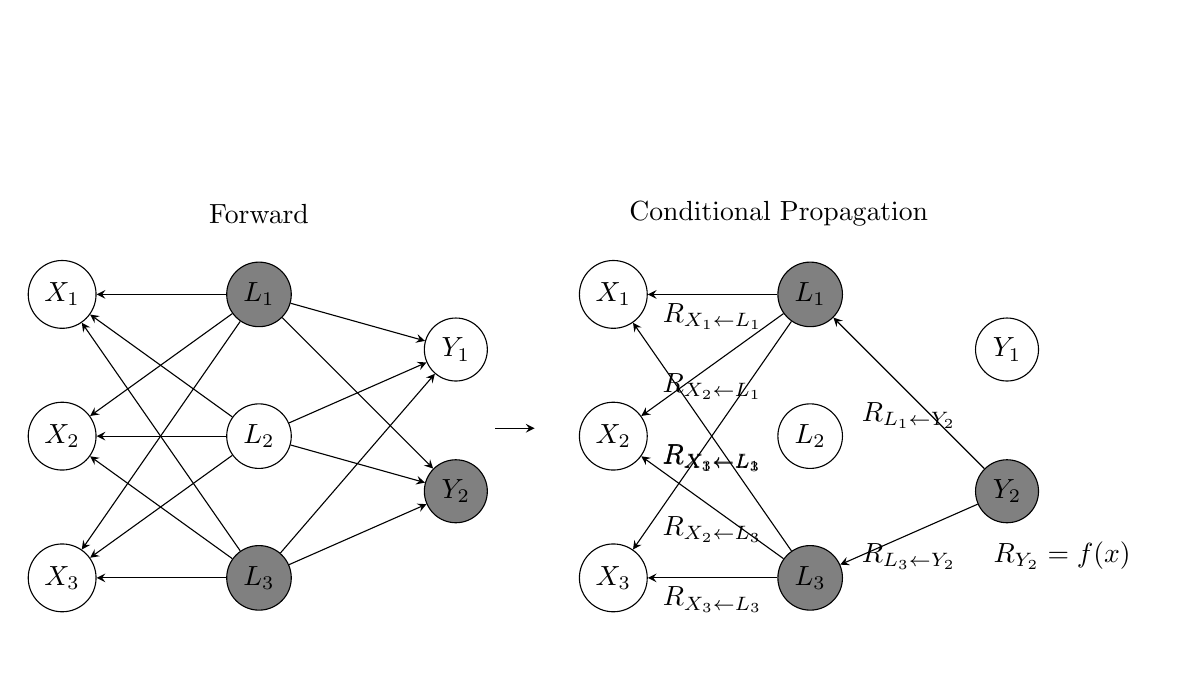
\begin{tikzpicture}[>=stealth,
            every node/.style={ draw, minimum size=8mm, align=center},]

        % First layer
        \foreach \x in {1,2,3} {
                \node [neuron] (X\x) at (0,{-\x* 1.8}) {$X_\x$};
            }
        \node [edgelabel]  (ti1) at (2.5,-0.5) {Forward};
        % Second layer
        \foreach \x in {1,2,3}{
                \pgfmathparse{\x==1 || \x ==3}
                \ifnum \pgfmathresult=1
                    \node  [neuron, conditioned]  (L\x) at (2.5,{-\x* 1.8}) {$L_\x$};
                \else
                    \node  [neuron]  (L\x) at (2.5,{-\x* 1.8}) {$L_\x$};
                \fi
            }

        % Last layer
        \foreach \x in {1,2} {
                \ifnum \x = 2
                    \node [neuron, conditioned]  (Y\x) at (5,{-\x* 1.8 - 0.7}) {$Y_\x$};
                    %\node [neuronlabel] at (Y\x.south) {$R_{Y_\x} = f(x)$};
                \else
                    \node  [neuron]  (Y\x) at (5,{-\x* 1.8 - 0.7}){$Y_\x$};
                \fi
            }

        % Connect nodes
        \foreach \y in {1,2,3}
        \foreach \x in {1,2,3}{
                \ifnum\x=\y
                    \draw[<-] (X\x) -- (L\y); 
                    %node[midway, edgelabel] {$R_{X_\x  \gets L\y}$};
                \else
                    \pgfmathparse{2 > \x-\y && 2 > \y-\x}
                    \ifthenelse{\pgfmathresult=1}{\draw[<-] (X\x) -- (L\y);}{}
                \fi
            }
        \foreach \x in {1,2,3}
        \foreach \y in {1,2}
        \draw[->] (L\x) -- (Y\y);

        \draw[->] (5.5,-3.5) -- (6,-3.5);

        % OTHER GRAPH
        % First layer
        \foreach \x in {1,2,3} {
                \node [neuron] (X\x) at (7,{-\x* 1.8}) {$X_\x$};
            }

        % Second layer
        \node [edgelabel]  (ti2) at (9.1,-0.5) {Conditional Propagation};
        \foreach \x in {1,2,3}{
                \pgfmathparse{\x==1 || \x ==3}
                \ifnum \pgfmathresult=1
                    \node  [neuron, conditioned]  (L\x) at (9.5,{-\x* 1.8}) {$L_\x$};
                \else
                    \node  [neuron]  (L\x) at (9.5,{-\x* 1.8}) {$L_\x$};
                \fi
            }

        % Last layer
        \foreach \x in {1,2} {
            \ifnum \x = 2
                \node [neuron, conditioned]  (Y\x) at (12,{-\x* 1.8 - 0.7}) {$Y_\x$};
                \node [neuronlabel] at (12.7,{-\x* 1.8 - 1.3}) {$R_{Y_\x} = f(x)$};
            \else
                \node  [neuron]  (Y\x) at (12,{-\x* 1.8 - 0.7}){$Y_\x$};
            \fi
        }

        % Connect nodes
        \foreach \y in {1,3}
        \foreach \x in {1,2,3}{
                \pgfmathparse{2 > \x-\y && 2 > \y-\x}
                \ifthenelse{\pgfmathresult=1}{\draw[<-] (X\x) -- (L\y)  node[midway, edgelabel] {$R_{X_\x  \gets L_\y}$};}{}
            }
        \foreach \x in {1,3}
        \foreach \y in {2}
        \draw[<-] (L\x) -- (Y\y) node[midway,align=center, edgelabel] {$R_{L_\x  \gets Y_\y}$};

    \end{tikzpicture}

    \caption{Left side: simple neural network forward pass with input layer X, one hidden layer L and output layer Y. Conditioning set $\theta = \{L_1, L_3, Y_2\}$ \\ Right side: only the relevance of the neurons matching the conditioning set is propagated back \\
    Result at input pixel $R_{X_2} = \sum_{j}  R_{X_2 \gets L_j} =  \sum_i \sum_{j} \cdot \frac{a_i w_{ij}}{\sum_h a_h w_{hj}} R_j \dots$ }
    \label{fig:crp_example_condition}
\end{figure}

\begin{itemize}
    \item some examples of usage:
          \begin{itemize}
              \item relevance scores for \textit{concepts} (=neurons)
              \item relevance maximization images
              \item conditioning on single concepts/ neurons ...?
              \item attribution graph
          \end{itemize}
\end{itemize}


\section{Causal Framework}
\subsection{Structural Causal Models}

\begin{itemize}
    \item Explain and define in detail Structural Causal Models
    \item neural networks could be seen as SCMs \cite{Chattopadhyay2019}
    \item but AI / neural networks in general do not care about causation and work through finding useful correlations
    \item and that is good this way, otherwise they would never find anything useful, statistics and correlations are great
    \item none-the-less the better we get at identifying spurious features the more causal methods might apply?
    \item it doesn't matter whether the network has found the actual causal reasons for its prediction, but explanations are a distinctively causal concept.
    \item and explanation asks how and why, so we want to know the cause of model predicting Y from X
    \item causal methods have started to be used for evaluation of xai
\end{itemize}

\subsection{Interpretation as Interventions}
???

\subsection{Data Generation Process}

Other?

\begin{itemize}
    \item Short introduction to causal effects    \item counterfactuals
    \item
\end{itemize}


\section{Evaluation of Explanations}
\subsection{Ground Truth Importance}
\begin{itemize}
    \item What are currently used ground truth importance measures for concepts or latent factors
    \item introduce Prediction Flip with formula or application to our use case
    \item R2 score with formula \cite{Sixt2020}
    \item mean logit change with formula
    \item make clear: human understanding is the ultimate goal, so user studies are the gold standard (but often not well done) but not feasible here
    \item relate to constant vector shift problem and how this might be measured
\end{itemize}
\subsection{CRP Concept Importance Measures}
\todo{need proper measure}
\begin{itemize}
    \item explain the measures i use to score how well the concepts are separated
    \item show theoretical basis
\end{itemize}
\subsection{Causally somehow? }